\section{The Specimen Data Refinery}
\label{ch8:the-specimen-data-refinery}

\subsection*{A canonical workflow framework and FAIR Digital Object
approach to speeding up digital mobilisation of natural history
collections}

A key limiting factor in organising and using information from physical
specimens curated in natural science collections is making that
information computable, with institutional digitization tending to focus
more on imaging the specimens themselves than on efficiently capturing
computable data about them. Label data are traditionally manually
transcribed today with high cost and low throughput, rendering such a
task constrained for many collection-holding institutions at current
funding levels.

We show how computer vision, optical character recognition, handwriting
recognition, named entity recognition and language translation
technologies can be implemented into canonical workflow component
libraries with findable, accessible, interoperable, and reusable (FAIR)
characteristics. These libraries are being developed in a cloud-based
workflow platform -- the `Specimen Data Refinery' (SDR) -- founded on
Galaxy workflow engine, Common Workflow Language, Research Object Crates
(RO-Crate) and WorkflowHub technologies. The SDR can be applied to
specimens' labels and other artefacts, offering the prospect of greatly
accelerated and more accurate data capture in computable form.

Two kinds of FAIR Digital Objects (FDO) are created by packaging outputs
of SDR workflows and workflow components as digital objects with
metadata, a persistent identifier, and a specific type definition. The
first kind of FDO are computable Digital Specimen (DS) objects that can
be consumed/produced by workflows, and other applications. A single DS
is the input data structure submitted to a workflow that is modified by
each workflow component in turn to produce a refined DS at the end. The
Specimen Data Refinery provides a library of such components that can be
used individually, or in series. To cofunction, each library component
describes the fields it requires from the DS and the fields it will in
turn populate or enrich. The second kind of FDO, RO-Crates gather and
archive the diverse set of digital and real-world resources,
configurations, and actions (the provenance) contributing to a unit of
research work, allowing that work to be faithfully recorded and
reproduced.

Here we describe the Specimen Data Refinery with its motivating
requirements, focusing on what is essential in the creation of canonical
workflow component libraries and its conformance with the requirements
of an emerging FDO Core Specification being developed by the FDO Forum.

\subsection{Introduction}\label{introduction-2}

A key limiting factor in organising and using information from physical
specimens curated in natural history collections is making that
information computable (`machine-actionable') and extendable. More than
85\% of available information currently resides on labels attached to
specimens or in physical ledgers \cite{Walton 2020}. Label data are commonly
transcribed manually with high cost and low throughput, rendering such a
task constraining for many institutions at current funding levels.
However, the advent of rapid, high-quality digital imaging has meant
that digitizing specimens, including their labels, is now faster and
cheaper \cite{ch8-2}. With initiatives such as Advancing Digitization of
Biological Collections (ADBC), integrated Digitized Biocollections
(iDigBio) and the Distributed System of Scientific Collections (DiSSCo)
\cite{ch8-3,ch8-4,ch8-5,ch8-6} aiming to increase the rate and accuracy of both mass and
on-demand digitization of natural history collections, the gap between
expectations of what should be digitally available and computable, and
what can be achieved using traditional transcription approaches is
widening. Modern, highly efficient workflow tools and approaches can
play a role to address this.

Collection digitization began towards the end of the 20th century by
typing basic data from labels into the collection (asset) management
systems of collection-holding institutions such as natural history
museums, herbaria and universities. Initially, this was to facilitate
indexing and cataloguing and locating the physical specimens, but with
the addition of photographic images of specimens and the public
availability of specimen data records, through data portals of the
institutions themselves as well as international data infrastructures
like the Global Biodiversity Information Facility (GBIF), such bodies of
data have been rapidly exploited for research \cite{ch8-7,ch8-8}. It has become
clear that widespread digitization of data about physical specimens in
collections and the advent of high-throughput digitization processes
\cite{ch8-9,ch8-10,ch8-11,ch8-12,ch8-13} is transforming and will radically further transform the
range of scientific research opportunities and questions that can be
addressed \cite{ch8-14,ch8-15}. Scientific conclusions and policy decisions
evidenced by digital specimen data enhance humankind's ability to
conserve, protect, and predict the biodiversity of our world
\cite{ch8-16,ch8-17}.

Harnessing technologies developed to harvest, organise, analyse and
enhance information from sources such as scholarly literature,
third-party databases, data aggregators, data linkage services and
geocoders and reapplying these approaches to specimens' labels and other
artefacts offers the prospect of greatly accelerated data capture in a
computable form \cite{ch8-18}. Tools of particular interest span the fields
of computer vision, optical character recognition, handwriting
recognition, named entity recognition and language translation.

Workflow technologies from the ELIXIR Research Infrastructure \cite{ch8-19},
including Galaxy \cite{Afgan 2018}, Common Workflow Language \cite{Crusoe 2022}, Research
Object Crates (RO-Crates) \cite{OCarragain 2019,Soiland-Reyes 2022} and WorkflowHub \cite{Goble 2021}, and
selected tools are integrated in a cloud-based workflow platform for
natural history specimens -- the `Specimen Data Refinery' \cite{Walton 2020} that
will become one of the main services to be offered by the planned DiSSCo
research infrastructure \cite{ch8-5}. The tools themselves, implemented with
findable, accessible, interoperable, and reusable (FAIR) characteristics
\cite{Wilkinson 2016} are packaged into canonical workflow component libraries
\cite{ch8-27}, rendering them reusable, and interoperable with one another.
FAIR Digital Objects are adopted as the common input/output pattern,
fully compatible with digital objects at the core of DiSSCo data
management \cite{ch8-28}.

The Refinery brings together domain-specific workflows for processing
specimen images and extracting text and data from images with canonical
forms for components and interactions between components that can lead
to improved FAIR characteristics for both the workflows themselves and
the data resulting from workflow execution.

FAIR Digital Objects (FDO) are created by packaging outputs of workflows
and workflow components as digital objects with metadata, a persistent
identifier, and a specific type definition against which operations can
be executed \cite{De Smedt 2020}. The Refinery uses two kinds of FDOs:

\begin{itemize}
\item
  \textbf{computable Digital Specimen (DS) objects} \cite{ch8-30} from DISSCo
  for the scientific input/output data that can be consumed/produced by
  workflows and other applications.
\item
  \textbf{workflow objects, implemented as RO-Crates} \cite{Soiland-Reyes 2022}, from
  ELIXIR gather and archive the diverse set of workflow process data --
  the digital and real-world resources, configurations and actions (the
  provenance) contributing to a unit of digitization or other work
  producing the Digital Specimen digital objects, allowing that work to
  be scrutinised and faithfully reproduced if necessary.
\end{itemize}

We first summarise related work before describing the problem to be
addressed by the Specimen Data Refinery. We then explain our Canonical
Workflows for Research (CWFR) approach using these FDOs in the design of
the SDR, the experimental setup, and results so far from the work in
progress. While future work will clarify full results and challenges of
implementing a robust, reliable, and easy-to-use production-capability
SDR, in this early report following SDR prototyping and
conceptualization, we focus on what we found to be essential in the use
of FDOs and CWFR canonical step libraries, and on the compliance of
canonical workflow (component) inputs and outputs with the requirements
of the FDO Framework \cite{bonino2019}.

\subsection{Related Work}\label{related-work}

\subsubsection{Workflows for processing specimen images and extracting data}\label{workflows-for-processing-specimen-images-and-extracting-data}

While natural history collections are heterogeneous in size and shape,
often they are mass digitized using standardised workflows \cite{ch8-9,ch8-10,ch8-11,ch8-12,ch8-13}.
In pursuit of higher throughput at lower cost, yet with higher accuracy
and richer metadata, further automation will increasingly rely on
techniques of object detection and segmentation, optical character
recognition (OCR) and semantic processing of labels, and automated
taxonomic identification and visual feature analysis \cite{Walton 2020,ch8-18}.

Although there is a great deal of variety among images of different
kinds of collection objects that are digitized (see Figure \vref{ch8:figure1}) there are
visual similarities between them. Most images contain labels, scale bars
and often, colour charts as well as the specimen itself. This makes them
amenable to improved approaches to object detection \cite{ch8-32} and
segmentation into `regions of interest' \cite{ch8-33} as precursive steps for
multiple kinds of workflows.

%% Evil footnotes again
\begin{figure}%[t]
  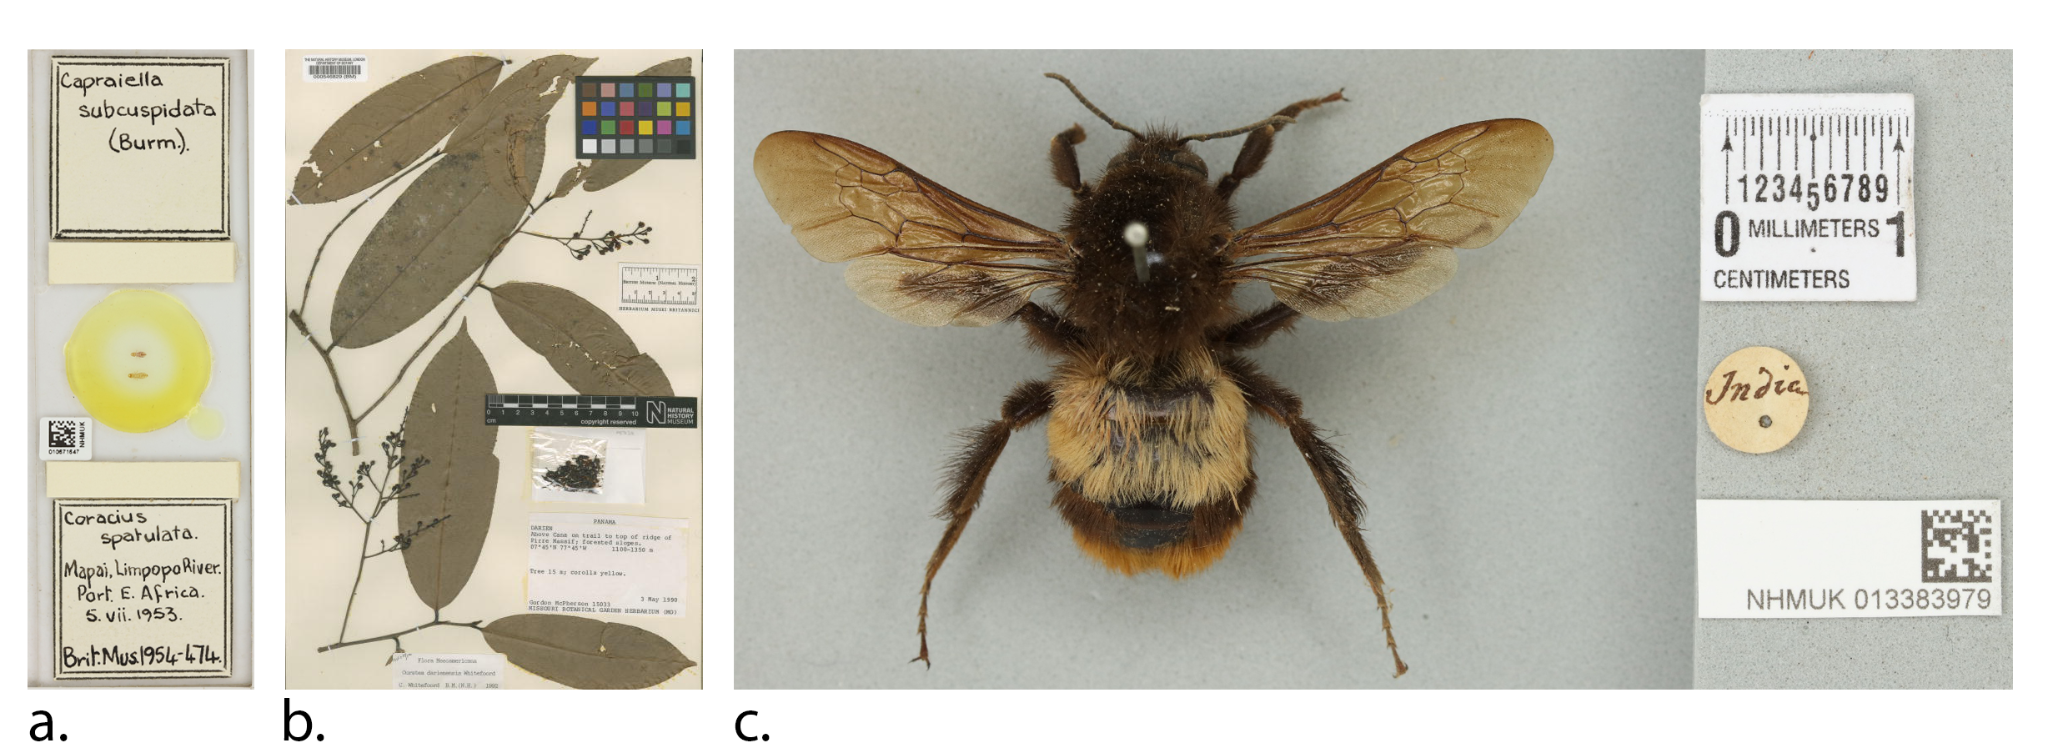
\includegraphics[width=\textwidth]{figures/ch08/figure1.png}
	\caption[A range of specimen images]{\textbf{A range of specimen images}. From the Natural History Museum, London, demonstrating the
  diversity of collection objects, which include handwritten, typed, and
  printed labels. (a) Microscope slide (NHMUK010671647)\footnotemark{},
  (b) Herbarium specimen (BM000546829)\footnotemark{},
  (c) pinned insect (NHMUK013383979)\footnotemark{}.}
  \label{ch8:figure1}
\end{figure}

% Evil goes her
\addtocounter{footnote}{-3}
\addtocounter{footnote}{1}\footnotetext{\url{https://data.nhm.ac.uk/object/c65d9a3c-d8f6-4fac-a418-05c3b697cece}}
\addtocounter{footnote}{1}\footnotetext{\url{https://data.nhm.ac.uk/object/be595f07-73c5-4764-a96c-8b377e3d1507}}
\addtocounter{footnote}{1}\footnotetext{\url{https://data.nhm.ac.uk/object/745febc7-8222-498a-9969-5f6b12f85ef3}}
%%

Segmentation, specifically, can be employed as an early step in a
workflow to send just the relevant region(s) of interest from an image
to later workflow steps. Not only does this decrease data transfer time
and minimise computational overheads but it can also substantially
increase the accuracy of subsequent OCR processing and semantic
recognition steps \cite{ch8-18}.

Much of the data about specimens is stored on their handwritten, typed
or printed labels or in registers/ledgers \cite{ch8-34}. Direct manual
transcription into local databases with manual georeferencing is the
primary method used today to capture this data. Potentially, OCR can
significantly increase transcription speeds whilst reducing cost;
although it sacrifices accuracy and disambiguation that are today
achieved with specialist knowledge provided by humans during the
process. Returning character strings from OCR is useful, but
semantically placing this data in its context as information specific to
natural history specimens and linking that back to the original physical
specimens is of much higher value, improving the utility of natural
history collections. Shortfalls in accuracy and disambiguation can be
made up by exploiting Natural Language Processing (NLP) advances such as
named entity recognition to identify text segments belonging to
predefined categories (for example, species name, collector, locality,
date) \cite{ch8-18}. Nevertheless, this only works well on a small proportion
of captured data in the absence of `human in the loop' input. To better
automate disambiguation of people's names, for example, access to other
contextual `helper' data are needed (e.g., biographical data in
Wikidata) as well as cross-comparison with other data from the specimen,
such as the date of collection and location \cite{ch8-35}.

Automated identification of species from images of living organisms has
achieved impressive levels of accuracy 
\cite{ch8-36,ch8-37,ch8-38,ch8-39,ch8-40,ch8-41} with techniques
translated to an increasing range of enthusiastically received consumer
applications for plant and animal identification using mobile phones
(e.g., \footurl{https://www.plantsnap.com/}{Plantsnap},
\footurl{https://www.picturethisai.com/}{PictureThis},
\footurl{https://www.inaturalist.org/pages/seek_app}{iNaturalist SEEK}).
Automated identification of \emph{preserved specimens}, however,
presents different challenges. Although identification might be made
more accurately because a specimen is presented in a standard manner,
separated from other organisms and the complexity of a natural
background, the loss of colour and distortion of the shape of the
organism arising from preparation and preservation processes can lead to
the loss of important identification clues that might be present on a
living example.

\subsubsection{Workflow management systems and canonical workflows
for
research}\label{ch8:workflow-management-systems-and-canonical-workflows-for-research}

A workflow chains together atomised and executable components with the
relationships between them to clearly define a control flow and a data
flow. Their significant defining characteristics are (i) abstraction,
through the separation of the workflow specification (the work to be
done) from its execution (how it is done), and (ii) composition whereby
the components can be cleanly combined and reused and workflows
themselves can be neatly packaged as components \cite{Atkinson 2017}. Workflow
management systems typically provide the necessary mechanisms for
explicitly defining workflows in a reusable way together with a workflow
engine that executes the workflow steps and keeps an accountable record
of the processing -- logging the codes executed and the data lineage of
the results. In the past decade there has been a rise in popularity in
both the development of WfMS and their use, driven by the increasing
scales of data and the accompanying complexity of its processing
\cite{Atkinson 2017}.

Workflow management systems typically vary in the features they provide
for supporting: workflow programming language and control flow
expressivity; data type management; code wrapping, containerisation and
integration with software management tools; exploitation of
computational architectures; availability of development and logging
tools; licensing and so on. Although several hundred kinds of such
systems exist \cite{ch8-43}, communities tend to cluster around a few popular
systems based on their ``plugged-in'' availability of data type
specialist codes, the catered-for skills level of the workflow
developers, and its documentation, community support and perceived
sustainability. For the Specimen Data Refinery, the Galaxy workflow
system \cite{Afgan 2018} in conjunction with Common Workflow Language (CWL)
\cite{Crusoe 2022} has been chosen. CWL is a workflow specification standard
geared towards supporting interoperable and scalable production
pipelines, abstracting away from the internal data structures of some of
the language-specific workflow systems.

Originally designed for computational biology and with many available
tool components, Galaxy \cite{Afgan 2018} supports multiple domains. Workflows
can be built by manually experimenting with data manipulations in a
`data playground' and subsequently converting histories of those to
workflows, or by a more traditional drag-and-drop composition approach.
New components can be created by wrapping existing programs, with
in-built dependency management and automated conversion to executable
containers. As such, Galaxy and CWL offer possibilities for a rich
canonical workflow component landscape with a workflow management regime
that can be both easily FAIR compliant and efficient internally
\cite{ch8-27}. The WorkflowHub, which facilitates CWL and enables workflows
to be registered, shared and published, is mutually coupled with Galaxy
so that workflows can be discovered in the Hub and immediately executed
in a public-use Galaxy instance.

In the context of the SDR, users can construct institution or
project-specific variants of digitization workflows to suit their
specific needs. As collections are heterogeneous, different specimen
types or specific sets of specimens are likely to have variations and
idiosyncrasies in the digitization and processing needed. Tools for
automated identification of specimens are likely to be taxon-specific,
and as such it seems likely that taxon-specific workflows will become
common. In addition, institutions have specific data exchange
requirements for their individual collection management systems.
Ensuring that workflows can be easily modified in a common environment
bridges the gap between community contribution to shared tooling and the
bespoke needs of specific institutions/collections.

Although computational workflows typically emphasize scalable automated
processing, in practice many also combine automation with manual steps.
This feature is also supported by Galaxy and CWL, allowing (for example)
manual geocoding and verification during the digitization process of the
locations where specimens were collected.

\subsubsection{FAIR Digital Objects}\label{fair-digital-objects-1}

Galaxy/CWL environments offer the possibility to integrate generic
digital object methods \cite{ch8-44,ch8-45,Kahn 2006} for the interactions between
workflow components, thus making them able to meet the need and ease the
burden of compiling FAIR compliant data throughout the research
lifecycle \cite{ch8-27}.

A digital object exhibiting FAIR characteristics is a FAIR Digital
Object \cite{De Smedt 2020} and is defined formally as ``a unit composed of data
and/or metadata regulated by structures or schemas, and with an assigned
globally unique and persistent identifier (PID), which is findable,
accessible, interoperable and reusable both by humans and computers for
the reliable interpretation and processing of the data represented by
the object''.

Supporting `FAIRness' internally and acting as glue between the steps of
canonical workflows, FDOs record and can represent the state of a
workflow, its inputs and outputs, and the component steps performed in a
comprehensive manner \cite{ch8-27}. Each FDO is anchored by a globally unique
and resolvable, persistent identifier (PID) (such as a DOI®, for
example) that clearly refers to one digital entity. The PID resolution
offers persistent references to find, access and reuse all information
entities that are relevant to access and interpret the content of an
FDO. In doing so, the FDO creates a new kind of machine-actionable,
meaningful and technology independent unit of information. This is both
immediately available and amenable for further use, as well as being
comparable to the role of the classical archival storage box when
necessary.

\paragraph{Computable Digital Specimens as a kind of FAIR Digital Object}\label{computable-digital-specimens-as-a-kind-of-fair-digital-object}

Digital Specimens (DS) are a specific class of FDO that group, manage
and allow processing of fragments of information relating to physical
natural history specimens. On a one-to-one correspondence a DS
authoritatively collates data about a physical specimen (i.e.,
information extracted and captured from labels by digitization
workflows) with other data -- often to be found from third-party sources
-- derived from analysis and use of the specimen.

openDS \cite{ch8-47} is the developing specification for open Digital
Specimens and other related object types, defining: 

\begin{itemize}
  \item The logical
  structure and content of Digital Specimen (DS), Basic Image Object (BIO)
  and other object types, and the operations permitted on them
  \item The
  handling rules and behaviors governing digital specimen object
  operations in general
  \item Serialization and packaging as
  JavaScript Object Notation (JSON) for lightweight data interchange
  between systems, sub-systems and components of systems (for which, read
  `workflow components' \cite{ch8-48}. 
\end{itemize}

openDS is essential to future FAIR
digitization of natural history collections and to Digital Specimens as
self-standing digital objects on the Internet, amenable to computer
processing. It contributes to the new transformative generation of FAIR
infrastructure and applications based on Digital Object Architecture
that is planned for the Distributed System of Scientific Collections
(DiSSCo) \cite{ch8-6,ch8-5,ch8-30} European research infrastructure.

Henceforth we refer to these as \textbf{openDS FDOs}.

\paragraph{FAIR packaging of research/workflow objects with RO-Crate}\label{ch8:fair-packaging-of-researchworkflow-objects-with-ro-crate}

The useful outcomes of research are not just traditional publications
nor data products but everything that goes into and supports an
investigative work or production pipelining activity. This includes
input and intermediate data, parameter settings, final outputs, software
programs and workflows, and configuration information sufficient to make
the work reproducible. Research objects \cite{Bechhofer 2013} are a general approach
to describing and associating all of this content together in a
machine-readable form so that it can be easily preserved, shared and
exchanged. Workflow objects are a specific subclass of research objects.

RO-Crate\footnote{Chapter \vref{ch5:packaging-research-artefacts-with-ro-crate}} \cite{OCarragain 2019,Soiland-Reyes 2022} has been established as a community standard to
practically achieve FAIR packaging of research objects with their
structured metadata. Based on well-established Web standards, RO-Crate
uses JSON-LD \cite{w3-json-ld} with \cite{schema.org} for its common metadata representation. It is extensible with
domain-specific vocabularies in a growing range of specializing RO-Crate
profiles, e.g., for domains such as earth sciences \cite{ch8-52}, biosciences
\cite{Goble 2021}; for object types such as data or workflow \cite{Bacall 2022}; or for
workflow runs). RO-Crate has been proposed for the implementation of
FAIR Digital Objects on the World Wide Web as a common representation of
the FDO Metadata objects foreseen by the FDO Framework \cite{Goble 2021,bonino2019}.
Combined with FAIR Signposting \cite{Van de Sompel 2022} for resolving persistent
identifiers (PID) to FDOs on the World Wide Web, these RO-Crates are
findable, accessible, interoperable, and reusable by machines to both
create and obtain the information they need to function.

Henceforth, we refer to \textbf{RO-Crate FDOs}.

\subsection{Problem Description}\label{problem-description}

\subsubsection{Automating digitization and capturing the process}\label{automating-digitization-and-capturing-the-process}


In the lengthy history of collectors and museums curating artefacts and
specimens, we see that there have been and always will be ambiguities,
uncertainties, and inaccuracies in interpretations of recorded
information and attached labels \cite{ch8-56}. The practices of different
collectors and curators vary and change over time. There are constraints
of the label medium itself arising from the specifics of accepted
preparation and preservation processes (e.g., tiny, handwritten labels
pinned to butterflies).

Although systematic digitization of label and other recorded data can
help to unify otherwise diverse information (e.g., species names,
locations) the digital process and the resulting digital specimen data
carry their own assumptions, simplifications, inconsistencies, and
limitations. Over time, tools and methods, workflows and data models all
evolve and improve. In particular, increasing automation for throughput
and accuracy often involves increased assistance from computers and
software.

Just as manual curation and improvement work implies the need for good
record keeping, so too does working digitally imply the importance of
ensuring that sufficient records are captured about the
computer-assisted digitization and curation processes (provenance).
These justify the produced digital specimen data and propagate credit
for work done to their analogue equivalents, and also allow
retrospective review, revision or recomputation of the produced data as
future needs, practices or knowledge change.

Globally, there is underinvestment and missing technical expertise for
wide-scale automated mass digitization. Sharing proven digitization
workflows via a repository or registry linked to an individual published
journal article presents significant barriers to re-use. Exploiting
hosted community environments -- in this case Galaxy and WorkflowHub --
for the deployed tooling lowers barriers and provides rapid and easy
access for institutions with limited capabilities and capacities for
digitization. Hosted workflows represent ``primacy of method'' for a
community evolving towards a new research culture that is becoming
increasingly dependent on working digitally and collaboratively
\cite{ch8-57,ch8-58}.

\subsubsection{Users, user stories and specimen categories}\label{users-user-stories-and-specimen-categories}

Initially, two kinds of users must be supported: digitizer technicians
and collections managers/curators. Five high-level user stories describe
and broadly encompass the functionality these users need:

\begin{enumerate}
\item
  As a digitizer, I want to construct a workflow from a set of
  predefined components, so I can use that workflow to digitize
  specimens to a predefined specification.
\item
  As a digitizer, I want to run one or many specimen images through a
  workflow so I can create new digital specimens.
\item
  As a collection manager/curator, I want to run one or many digital
  specimens through a workflow to enrich my digital specimens with
  further data.
\item
  As a collection manager/curator, I want to view the metadata of a
  digitization workflow run so I can understand what happened on that
  run.
\item
  As a digitizer, I want to export the output of a digitization run, so
  I can consume the output of a digitization run into my institution's
  collection management system.
\end{enumerate}

To prove the SDR concept, three categories of preserved specimen types
have been selected to be supported initially: herbarium sheets,
microscope slides and pinned insects (see Figure \vref{ch8:figure1}).

\subsection{The FDO and CWFR approach in the Specimen Data Refinery}\label{the-fdo-and-cwfr-approach-in-the-specimen-data-refinery}

Workflows will be designed to support the user categories and stories
given above. The performance of the SDR will be evaluated against these
specimen types, eventually using several thousand different specimen and
label images. This is in anticipation of SDR becoming part of the
pivotal technology to achieve high rates of mass FAIR digitization
expected through the planned DiSSCo research infrastructure \cite{ch8-6,ch8-5,ch8-30}.

\subsubsection{FDO types}\label{ch8:fdo-types}

In the Specimen Data Refinery (see Figure \vref{ch8:figure2}) the role of openDS FDOs is
planned as the basis for the primary workflow inputs and outputs, and
for data transfer and interactions between components within SDR
workflows. A single openDS FDO submitted to the beginning of the
workflow (or a \emph{de novo} digitization that is immediately wrapped
as a new openDS FDO) becomes modified by each workflow component to
produce an incrementally refined openDS FDO. FDOs are acting as the unit
of data communication between canonical workflow components, in that
each step is immediately creating an FDO with associated FAIR compliant
documentation.

\begin{figure}%[t]
  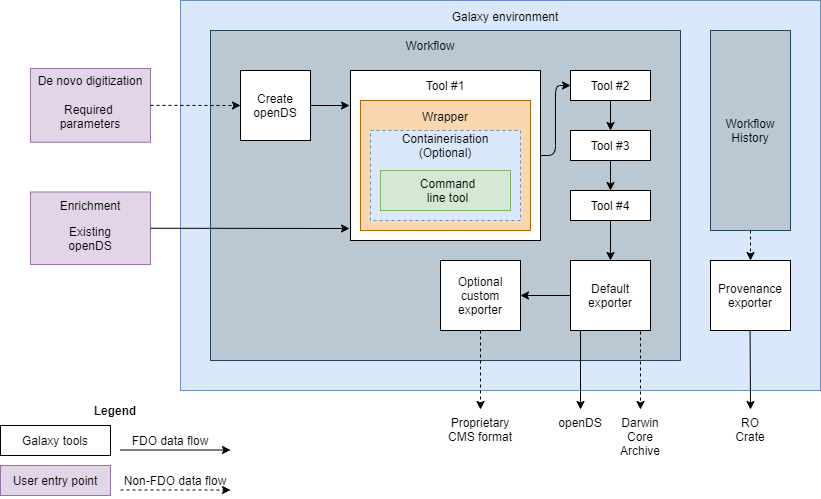
\includegraphics[width=\textwidth]{figures/ch08/figure2.png}
	\caption[CWFR approach]{\textbf{CWFR approach}. Adopted for the SDR as a Galaxy 
  workflow management system
  implementation with `\emph{de novo} digitization' and `enrichment' entry points.}
  \label{ch8:figure2}
\end{figure}


RO-Crate FDOs capture two aspects of a workflow:

\begin{enumerate}
\item
  A \textbf{Workflow-RO-Crate} contains the workflow definition, the
  computational tools and configuration, graphical image of the
  workflow, etc; this is the \emph{method} registered in the WorkflowHub
  and activated in the Specimen Data Refinery for execution.
\item
  A \textbf{Workflow-Run-RO-Crate} references (a) and records the
  details of a specific computational workflow run and its runtime
  information, with relations to the used and generated FDOs. This
  captures the digitization provenance that is generated as the openDS
  FDO makes its journey through a workflow.
\end{enumerate}

The final step in SDR workflows can be a data exporter tool, allowing
users to export the entire openDS object as is, or to convert and export
it in another format, such as CSV, DarwinCore Archive, etc. This
reconfigurable nature of data export allows users to define their own
transformer function to allow export to match formats specific to
specific collection management systems in use by their institution, such
that refined data can be repatriated. The provenance exporter transforms
Galaxy workflow history data into a Workflow-Run-RO-Crate FDO.

All FDO types are serialized as JSON.

\subsubsection{Canonical components}\label{canonical-components}

Each workflow component from a canonical library (to be built,
illustrated as tools \#1 - \#4 in figure \ref{ch8:figure2}) describes what attributes it
requires from the openDS FDO to be able to function, and the attributes
it will in turn populate or enrich. The interface between the component
and the openDS FDO is formed by the wrapper (orange in figure \ref{ch8:figure2}) around
the (optionally) containerized command-line tool (blue/green in figure
2). Canonical components can be used individually, or in series. The
openDS FDO data flows between components will always be of the same
type, being modified as the workflow proceeds.

This allows tools to function both as standalone components and as part
of any sequence of chained tools, provided that the specific openDS FDO
attributes required for a tool to work are pre-populated. This keeps the
SDR flexible and customisable for different digitization pipelines.

Two entry points are provided for users of the SDR. One is named as the
`\emph{de novo} digitization' entry point (figure \ref{ch8:figure2}) fulfilling the
needs of user story (2) where specimens are being newly digitized for
the first time. The second entry point, named as the `enrichment' entry
point (figure \ref{ch8:figure2}) fulfils the needs of user story (3) where an existing
openDS FDO (or reference to it) can be provided to the SDR as part of
the input data.

In parallel to manipulating openDS FDOs, the Refinery gathers the
minimum inputs and workflow components required to produce deterministic
output and produces a Workflow-Run-RO-Crate FDO.

\subsection{Experiments and analysis}\label{experiments-and-analysis}

\subsubsection{Experimental workflows}\label{experimental-workflows}

The workflows of the SDR compose different functional components
according to specific need: image segmentation, barcode reading, optical
character recognition, text contextualisation/entity recognition,
geocoding, taxonomic linkage, people linkage, specimen condition
checking, automated identification, and data export/conversion. Broadly
speaking there are two main kinds of workflow: (i) specimen workflows,
where the specimen itself is analysed for morphological traits, colour
analysis, condition checking and automated identification; and (ii) text
and label workflows, where handwritten, typed or printed text from the
image is read, named entities are classified, then linked to identifiers
or enhanced through post processing.

Both kinds of workflow can begin with initial openDS object creation
based on the submission of specimen image files and accompanying input
parameters through a forms-based user interface (\emph{de novo}
digitization entry point); or, alternatively, a pre-existing openDS
object with accompanying image object(s)can be supplied as the input
(enrichment entry point). Both kinds of workflow also rely on the image
segmentation component as the precursor for subsequent workflow steps.
Similarly, and if needed both kinds might use a format conversion and
export component as their final step; for example, if an openDS FDO is
not a natively compatible output for the next consuming application.

Although not within the scope of the present proof-of-concept, other
more precise workflows for enhancing specific aspects of existing
records can be foreseen. There are many specimen records, for example
where locality text, although digitally available, is not yet geocoded.
There are records with unlinked or ambiguous collector names that could
be linked/disambiguated; and records where unknown specimens still need
identifying.

\subsubsection{Experimental data and evaluation}\label{experimental-data-and-evaluation}

\paragraph{Evaluation images datasets}\label{evaluation-images-datasets}

The Refinery will be evaluated using sets of images, each composed of at
least 1,000 unique specimens for each of the three categories of
preserved specimen types: herbarium sheets, microscope slides and pinned
insects. For herbarium sheet images we will reuse an existing benchmark
dataset of 1,800 herbarium specimen images with corresponding
transcribed data \cite{ch8-59}. For microscope slide and pinned insect
specimen images similar evaluation datasets will be prepared against the
same label characteristics: written in different languages; printed or
handwritten; covering a wide range of dates; both type specimens and
general collections and will provide specimens from different families
and different parts of the world. Each test dataset set will be composed
of images from different institutions to ensure representation of
heterogeneity. For the present proof of concept, we limit the scope to
Latin alphabet languages. These datasets will also be used to train
Refinery models for use in tools (e.g., segmentation, named entity
recognition, object/feature detection). All the datasets will be made
publicly available with documentation.

\paragraph{Component functional tests}\label{component-functional-tests}

Galaxy has a built-in functional test framework. Tools intended to
become components of an SDR canonical library (actually, a Galaxy
ToolShed repository) will need to pass previously defined tests within
this framework. These tests, based on pre-supplied openDS FDO input and
output files containing the properties expected to be populated by the
tool, include validating a tool's own openDS FDO outputs by comparison
against the expected output file. It will be necessary to register
openDS FDOs as Galaxy custom data types.

\subsection{Results}\label{results}

openDS FDOs are the core data object at the heart of the SDR, playing
not only the workflow input/output role but acting also as a common data
structure between tool steps within the workflow. Users can launch the
workflow with either an openDS object, for further augmentation by the
SDR, or they can complete a form with the specimen information, which is
then converted to an openDS object before the workflow proper begins.

Each SDR Galaxy tool defines the properties it requires in JSONPath
syntax \cite{ch8-60}. The wrapper validates that these properties exist in
the openDS object, plucks them from the openDS JSON, makes them
available as named parameters, and passes these through to the tool
processing (via either a Docker or Python command line). The wrapper
validates the input openDS against the openDS schema, the tool performs
its processing and updates the openDS, and the wrapper validates the
changed openDS against the schema before writing to disk. For the
prototypical SDR, a static, local version of the openDS schema is used.
Future iterations will use referenceable versions of the openDS schema,
allowing for schema changes and for tools to validate their data input
and outputs against versions of the schema.

On ingestion, every openDS is assigned a persistent identifier, ensuring
unambiguity and referential integrity for every processed object. In
production, DOIs will be minted by the DiSSCo service; for the
proof-of-concept Handles with prefix \texttt{20.5000.1025/} will be
used.

\subsection{Discussion}\label{ch8:discussion}

\subsubsection{What is being achieved?}\label{ch8:what-is-being-achieved}

The design of the Specimen Data Refinery uses two kinds of FAIR Digital
Object -- openDS FDOs and RO-Crate FDOs. Each plays a role to ensure
`FAIRer' automated digitization for natural history specimens and
associated provenance capture:

\begin{itemize}
\item
  openDS FDOs act both as the input/output interface of a workflow and
  as the common intermediary pattern (canonical state) between steps
  within a workflow. They comply with DiSSCo data management principles
  and needs as outlined in the DiSSCo Data Management Plan \cite{ch8-28}
  allowing specimen data to be processed and extended in a fully FAIR
  manner \cite{ch8-6}.
\item
  RO-Crate FDOs record both the workflow definition and information
  about its configuration (shared as a method object) together with the
  details and context of the work done during a workflow run; details
  that are captured proprietarily within the adopted Galaxy environment
  and transformed to a common pattern (as another kind of canonical
  state) of provenance for later scrutiny and reproducibility of the
  work. These kinds of Research Objects \cite{Bechhofer 2013} are an established
  mechanism whereby computational methods become first-class citizens
  alongside data, to be easily shared, discussed, reused and repurposed
  \cite{ch8-57}.
\end{itemize}

Both kinds of FDO are essential. They complement one another to support
implementation of the FAIR principles, especially the interoperable and
reusable principles by making workflows self-documenting. This renders
automated whole processes (or fragments thereof) for digitizing and
extending natural history specimens' data as FAIR without adding
additional load to the researchers that stand to benefit most from that
\cite{ch8-27}. Each FDO type originates from different Research
Infrastructures (ELIXIR, DiSSCo) with different implementation
frameworks. Yet, they interoperate effectively due to their clear roles,
common conceptual model and separation of concerns.

\subsubsection{Different FDO implementations working together}\label{ch8:different-fdo-implementations-working-together}

openDS FDOs have their heritage in distributed digital object services
\cite{Kahn 2006} and are implemented through Digital Object Architecture (DOA)
\cite{ch8-62} with Digital Object Interface Protocol (DOIP) \cite{DONA 2018}, Digital
Object Identifier Resolution Protocol (DO-IRP) \cite{rfc3652}, and
recommendations of the Research Data Alliance \cite{ch8-65}. Serialized as
JSON, they are machine-actionable and compatible with established
protocols of the World Wide Web.

RO-Crates are native to the World Wide Web, based on established web
protocols, machine-readable metadata using Linked Data Platform methods
\cite{ch8-66}, JSON-LD and Schema.org \cite{Bechhofer 2013}, and community-accepted
packaging mechanisms such as BagIt. This makes RO-Crates straightforward
to incorporate into pre-existing platforms such as Galaxy and data
repositories such as Zenodo and DataVerse.

Both kinds of FDO use Persistent identifiers (PID), allowing instances
to be both uniquely identified and their location to be determined;
RO-Crates, as web natives, use URIs whereas openDS, as DOA objects, use
Handle PIDs. Instances of both kinds are described by metadata and
contain or reference data.

RO-Crates are self-describing using a metadata file and use
openly-extensible profiles to type the Crates (profile-typing) to set
out expectations for their metadata and content. openDS uses an
object-oriented object typing and instance approach to define the
structure and content of data/metadata. Complex object types are
constructed from basic types, an extension-section basic type. Both
approaches seek to avoid locking objects into repository silos, ensuring
that FDO instances can be interpreted outside of the contexts in which
they were originally created/stored.

Structurally and semantically openDS FDOs and RO-Crate FDOs are
potentially isomorphic, although at different granularity levels. Their
main difference is in method calling. As a DOA object, openDS would
expect to respond to type-specific method calls if these were
implemented. RO-Crates delegate actionability to applications that
interpret their self-describing profile.

Within the SDR the two kinds of FDO fulfill distinct and interlocking
roles for data (openDS) and self-documented method (RO-Crate) so their
different forms is not an issue. In future there may be a need to map
and convert between the approaches (e.g., for reconstructing past
processing), which would be assisted by the common FDO conceptual model
\cite{bonino2019}.

\subsubsection{Key domain challenges ahead}\label{key-domain-challenges-ahead}

For a digitized specimen to conform to FAIR principles, its data must be
linked to a vocabulary of terms, but choosing a single vocabulary is
likely to cause interoperability issues when cross-linking to resources
using another vocabulary, for example Darwin Core, Schema.org, or Access
to Biological Collection Data (ABCD). Whilst concepts can be mapped
across vocabularies (for example, using Simple Knowledge Organization
System (SKOS) matching), such an effort might rapidly become overly
complex and cumbersome, as the challenge of the Unified Medical Language
System (UMLS) demonstrates. The challenge remains - how is such a
mapping exercise maintained at a `just enough' level?

Different Earth Science domains have different use cases for digital
records. A digital record produced for biodiversity research is likely
to have different granularity, understanding and focus to one produced
for climate science. It remains to be seen if a single FAIR Digital
Object definition could be produced to satisfy multiple domains, and if
different objects could be produced for different domains, what would
they look like; and would this hinder future cross-compatibility?

The openDS FDO type produced by the SDR is a new object format for the
natural history domain that is foreseen to become an adopted standard
over time. Institutional collection management systems will need to be
upgraded before they can consume the FDO outputs from the SDR. Early
adopters may need assistance to produce SDR exporters matching
proprietary ingestion formats. For an interim period, there may be a
need for the SDR to output today's widely used Darwin Core Archives
format in parallel.

As the functional requirements of the SDR are emergent, a minimum viable
product has been scoped, but this should be contrasted with the notion
of a useful product. An MVP is a prototype; a tool to get a project off
the ground with enough features to be usable by early adopters, and to
build on to learn user requirements. But it is not intended to meet the
day-to-day requirements of all users. To nurture future development,
care must be taken to continue involving key stakeholders in eliciting
further requirements to make the SDR useful for the widest range of
users, and from there, develop a rich, configurable tool to allow simple
uptake and provide utility for resource-poor collections.

\subsection{Conclusion and Future Work}\label{conclusion-and-future-work}

The Specimen Data Refinery is likely to garner widespread interest
across the Natural History community. Whilst the promise of a scalable,
community-driven digitization platform is tantalising for many natural
history professionals, the Specimen Data Refinery project is still in
its early stages, and, as discussed above key challenges lie ahead.

Although natural history collections are generally catalogued by the
taxonomic identity of the curated object, there remains a large
historical backlog of unidentified specimens. The Meise Botanic Garden
(BE), for example, has an estimated 4 million specimens with at least
11\% not yet identified to species level. Furthermore, it is calculated
that half of the World's estimated 70,000 plant species yet to be
described have already been collected and are waiting in collections
still to be `discovered' \cite{Crusoe 2022}. The same is likely to be true for
other groups of organisms, especially insects. Unnamed specimens tend to
have lowest priority for digitization and their data are rarely shared.
Machine learning as canonical steps in SDR workflows presents a
tremendous opportunity to put an identification on these specimens and
potentially, to triage them for further taxonomic investigation.


